\documentclass[12pt]{article}

% Package lists
\usepackage{pythonhighlight}
\usepackage{solarized-dark}
\usepackage{geometry}
\usepackage{graphicx}

% Configurations
\geometry{margin=1cm, bottom=2cm}

\begin{document}
  \title{Report Lab 2}
  \author{Nguyen Tien Duc - ITITIU18029}
  \maketitle
  \part{Bisection vs False-Position}
    \section*{Bisection}
      \subsection*{Code}
        \inputpython{1a.py}{0}{48}
      \subsection*{Running}
        \begin{center}
            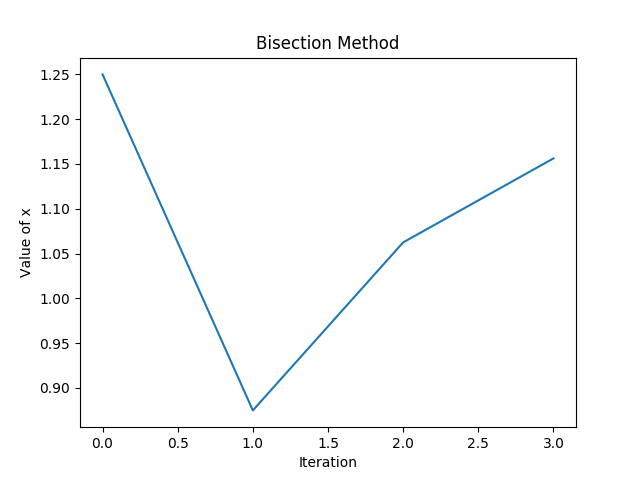
\includegraphics{BisectionGraph.png}
            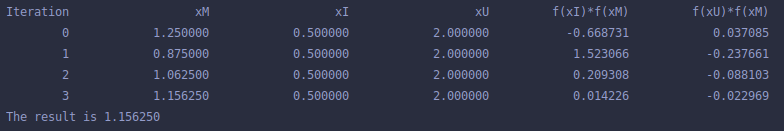
\includegraphics{BisectionResult.png}
        \end{center}
    \section*{False-Position}
      \subsection*{Code}
        \inputpython{1b.py}{0}{42}
      \subsection*{Running}
        \begin{center}
          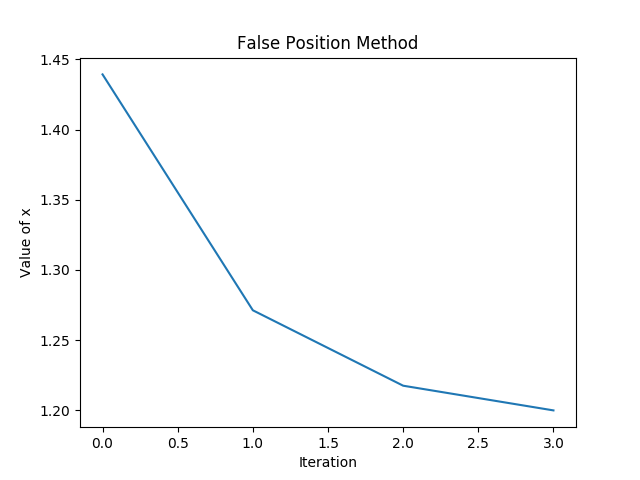
\includegraphics{RegulaFalsiGraph.png}
          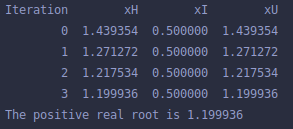
\includegraphics{RegulaFalsiResult.png}
        \end{center}
      \subsection*{Comment}
        This exercise showed right away that false-position method is better than bisection method.\\
        \begin{itemize}
          \item The first thing to notice is that the true value is 1.1912, which is much closer to the result of
          the false-position method after 3 iterations.
          On the other hand, the same number of iterations of bisection method only return a result that is
          accurate to the first decimal place.
          \item Secondly, the algorithm for false-position method is shorter, simpler, requires less computations and
          comparisons as showed.
          \item False Position likes to stick to one end for many iterations.
          \item This implementation is just a raw one, there are even faster ways to implement false-position method.
          \item Though false-position method is usually faster than bisection method.
          With certain complex functions, it can be still as slow as bisection method.
        \end{itemize}
        In conclusion, both are very old methods to find roots.\\
        However, due to the advantages of false-position method, some versions of it is still in use.\\
        Nevertheless, in reality, most people will switch to Newton's method or even Secant Method as those methods
        can usually do a better job than both false-position and bisection methods.
  \part{Fixed-Point Iteration vs Newton-Raphson}
    \section*{Fixed-Point Iteration}
      \subsection*{Code}
        \inputpython{2a.py}{0}{52}
      \subsection*{Running}
        \begin{center}
          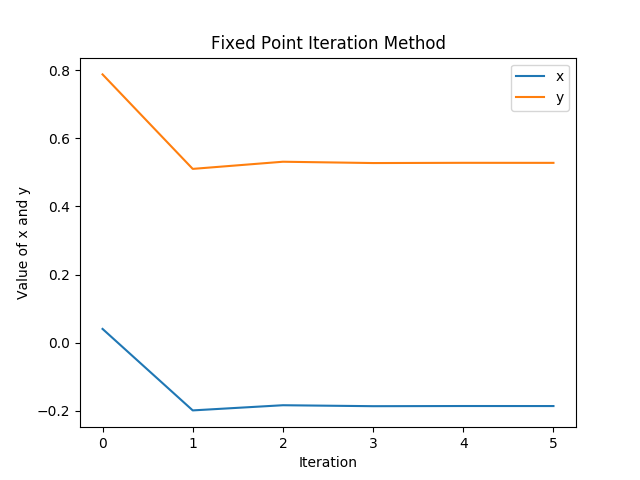
\includegraphics{FixedPointIteration.png}
          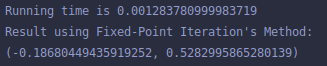
\includegraphics{FixedPointResult.png}
        \end{center}
    \section*{Newton-Raphson}
      \subsection*{Code}
          \inputpython{2b.py}{0}{90}
      \subsection*{Running}
      \begin{center}
        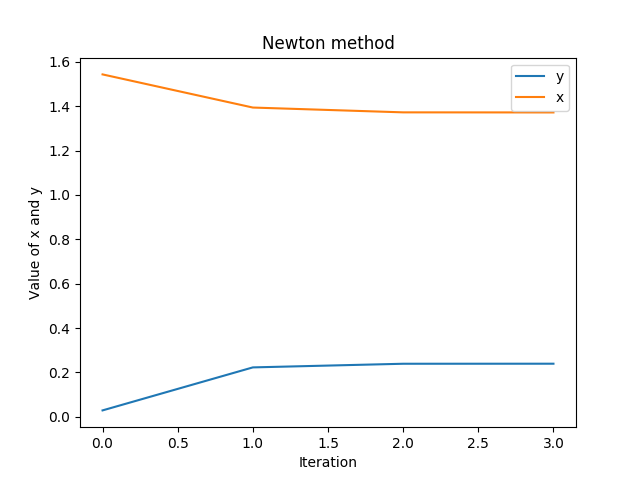
\includegraphics{NewtonRaphson.png}
        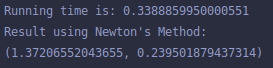
\includegraphics{NewtonRaphsonResult.png}
      \end{center}
      \subsection*{Comment}
        As the running time showed, Newton-Raphson method for solving system of non-linear
      equations is much slower compared to fixed-point iteration.
        However, the main advantage is the ability to solve bigger, more complex systems which
      is hard to show due to the simplicity of the system of equations given in the lab session. \\
        In conclusion, each method has their own advantages, thus they should be chosen wisely based
      on each particular function.
  \end{document}